% !Mode:: "TeX:UTF-8"
%此为第一章节。
%[h]为hear代码所在位置,\caption为表注题注,\cref{}引用图表公式章节等,\cite为引用参考文献,\subfloat子图,\label标签,\begin{figure}图片环境,\begin{table}表格环境,\begin{equation}公式环境,\toprule三线表顶线,\cmidrule三线表中线,\bottomrule三线表底线,\begin{theorem}定理,\begin{proof}证明,\begin{corollary}推论,\begin{lemma}引理

\chapter{绪论}\label{ch:1}
\section{节标题}

随着人工智能和第五代移动通信技术等系统技术的发展\cite{Lau_2022},推动着半导体行业在移动便携设备、高性能计算机、自动驾驶、物联网和大数据等应用领域的发展\cite{Lau_2022},同时也推动着电子芯片向着小型化和高集成化方向发展快速发展\cite{Sadique.Murtaza.ea_2022}。
在过去的几十年里处理器上的晶体管数量依照摩尔定律\cite{Tan.Du.ea_2021}的预测呈现出指数级的增长趋势,如这张50年间的微处理器的发展趋势图(\cref{fig:processor-trend})所示。
……

\subsection{小节标题}
\subsubsection{小小节标题}

\section{图片排版示例}
\subsection{单图排版示例}

\begin{figure}[htb]
    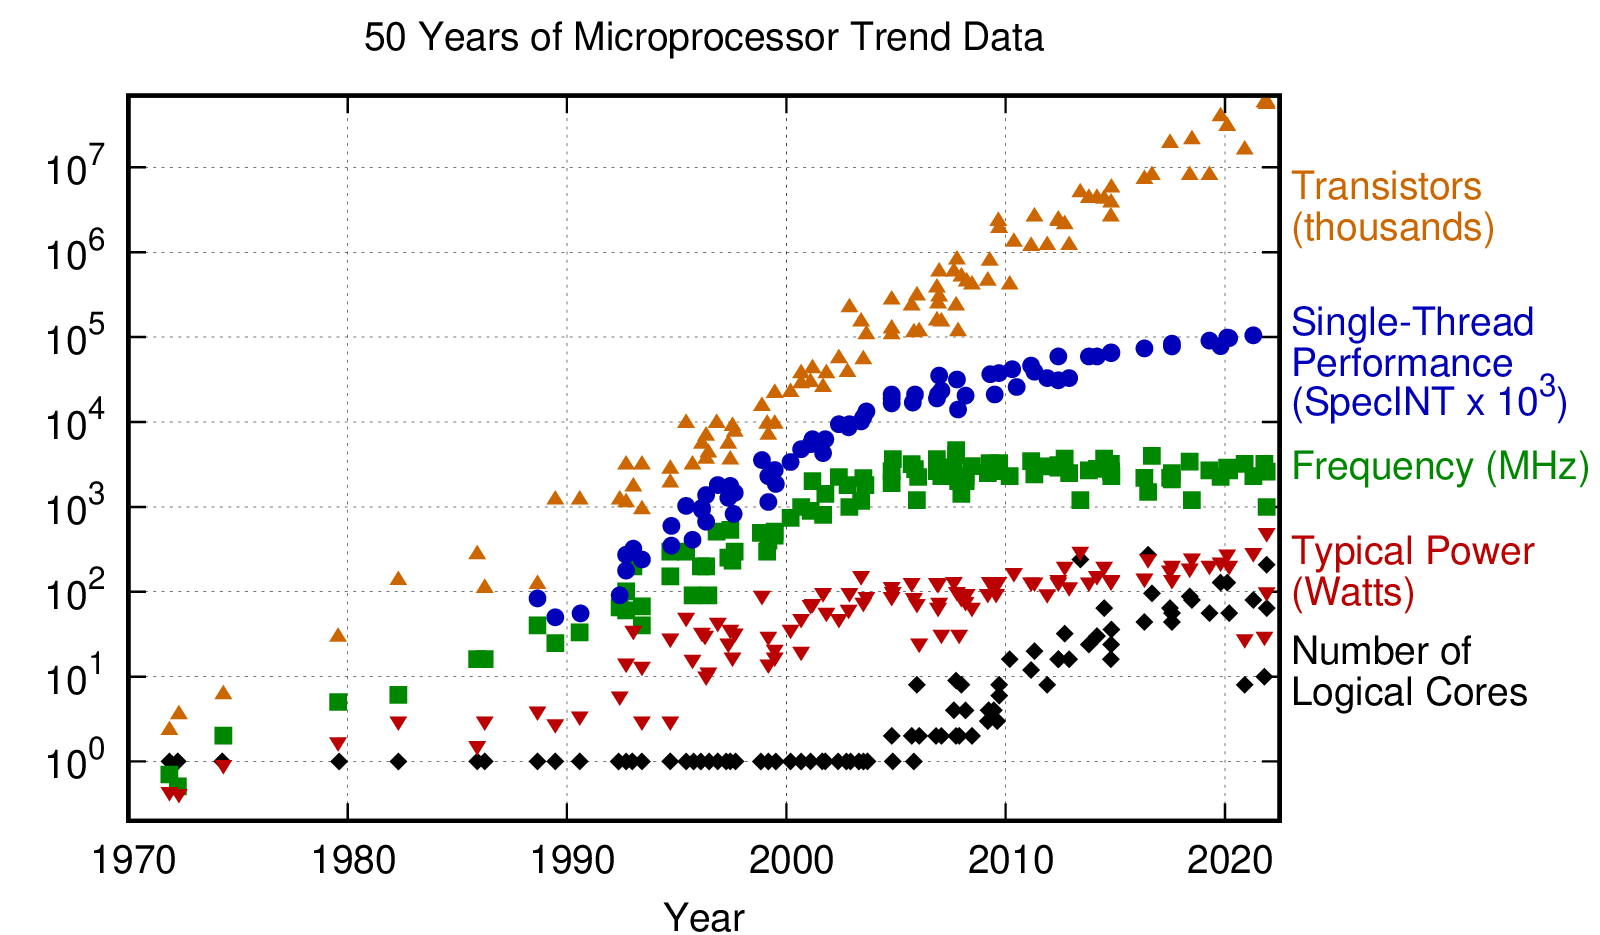
\includegraphics[width=0.8 \textwidth]{50-years-processor-trend.png}
    \caption[处理器发展]{近50年微处理器发展趋势} % 中括号中内容为插图索引中显示内容,可在题注内容过长时使用
    \label{fig:processor-trend}
\end{figure}

\subsection{多图排版示例}
同一行中的子图之间要留有空间,不要占满!否则会自动换行!

子图之间空一行表示换行。

\begin{figure}[htb]
    \subfloat[改进前的结构]{
        \label{fig:Unimproved-cooling-structure}
        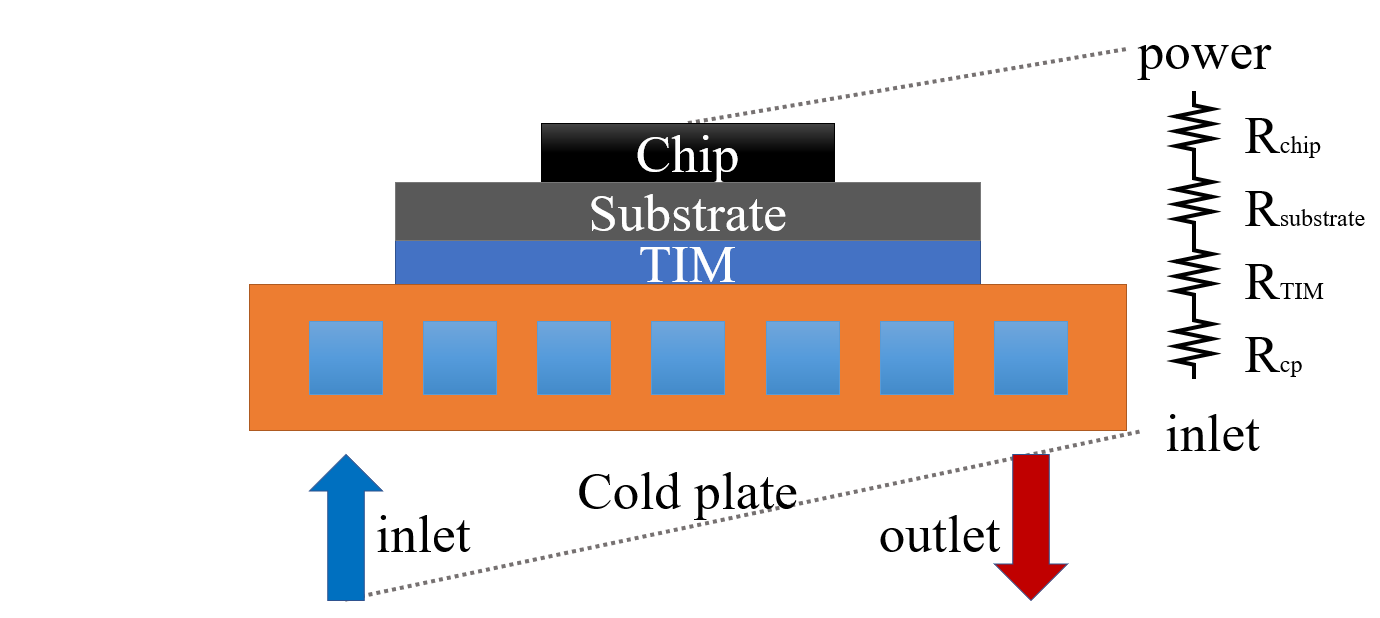
\includegraphics[width=0.45\linewidth]{Unimproved-cooling-structure.png}}
    \subfloat[基板内进行微通道散热]{
        \label{fig:LTCC-Microchannels}
        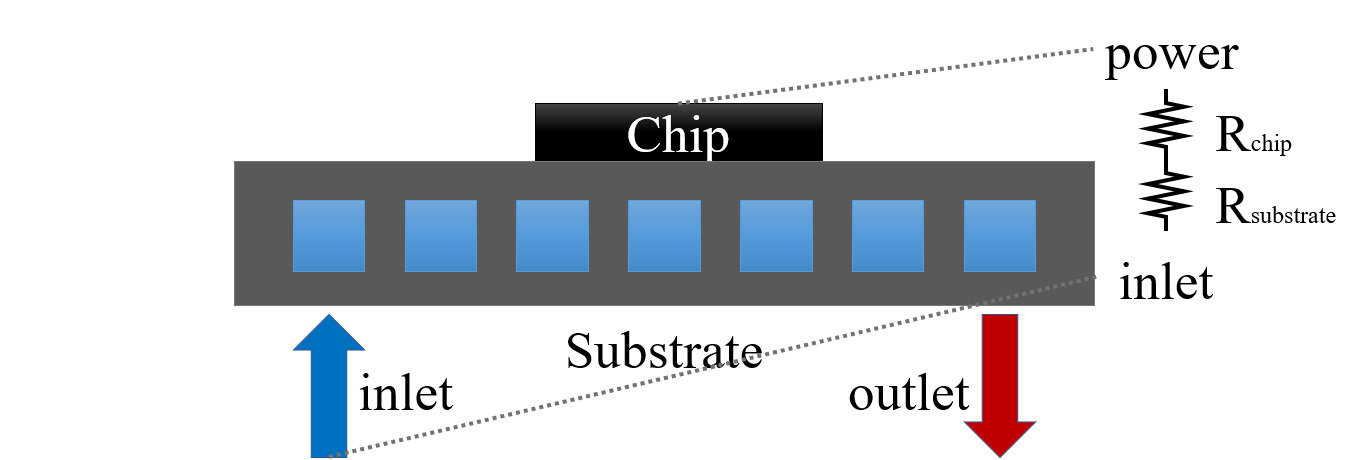
\includegraphics[width=0.45\linewidth]{LTCC-Microchannels.png}}

    \subfloat[嵌入散热模块]{
        \label{fig:Embedded-cooling-module}
        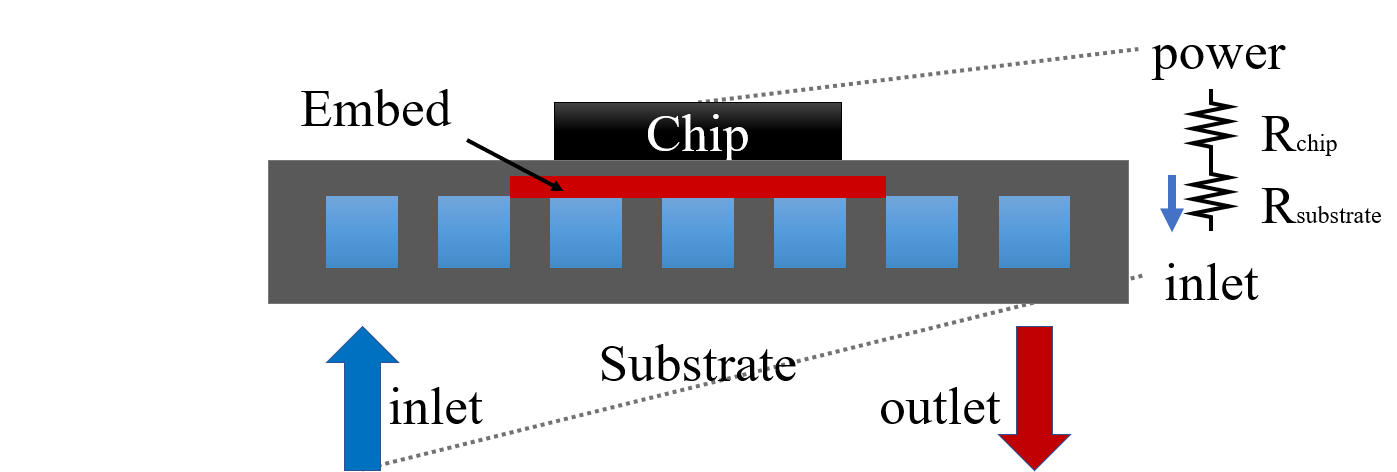
\includegraphics[width=0.45\linewidth]{Embedded-cooling-module.png}}
    \subfloat[带针鳍或肋的嵌入式散热模块]{
        \label{fig:Rib-pin-fin}
        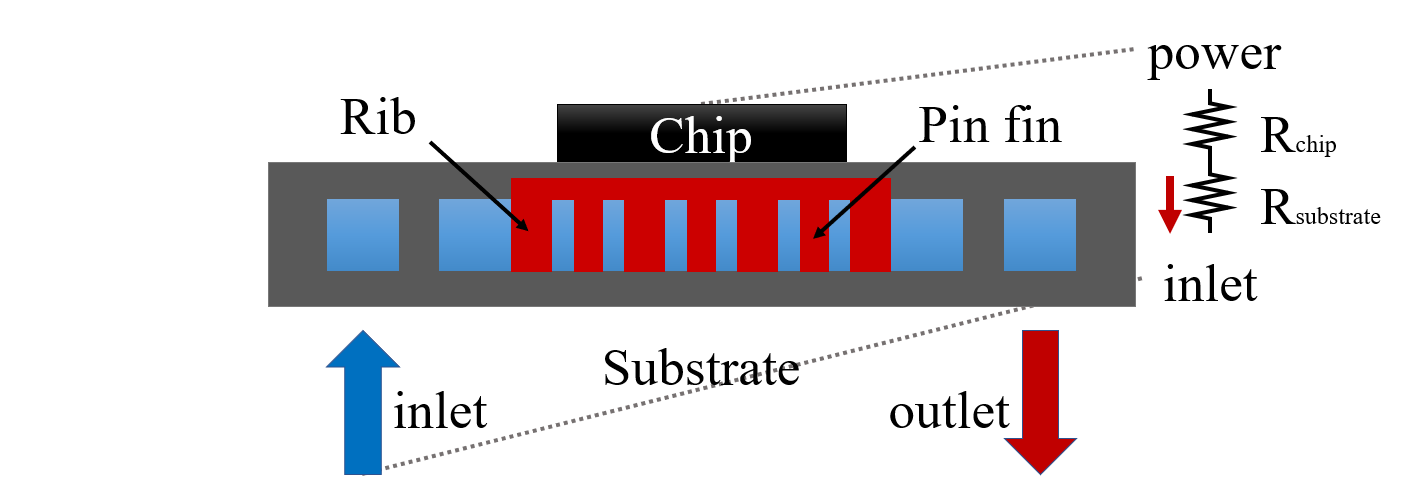
\includegraphics[width=0.45\linewidth]{Rib-pin-fin.png}}
    \caption{三种强化传热途径示意图}
    \label{fig:Three-enhanced-heat-transfer-paths}
\end{figure}


\section{本论文的结构安排}
\cref{ch:1}:绪论。本章主要分为……。

\cref{ch:2}:相关理论基础及结构设计要求与思路。本章主要分为……。

\cref{ch:3}:基于嵌入式散热模块的微通道流动与传热性能研究。本章研究了几种……。

\cref{ch:4}:基于嵌入式散热模块的微通道多目标优化分析。本章在\cref{ch:3}完成基于……。

\cref{ch:5}: 基于MC-RPF的多热源散热结构设计分析及压降优化。本章在\cref{ch:4}完成MC-RPF多目标优化……。

\cref{ch:6}:全文总结与展望。本次研究工作进行总结,并根据全文研究过程中……。


